
\documentclass{article}
\usepackage[utf8]{inputenc}
\usepackage{pgfplots}
\pgfplotsset{compat=1.18}
\usepackage{parskip}  % This will help for paragraph spacing, if needed
\begin{document}

\section*{\textbf{CS280 SPRING 2024 COURSE ASSESSMENT}}
Instructor \\
\\
\textbf{Part I - Performance Indicators, student outcomes and levels of focus.} \\
\\
CS5-R : Function effectively as a member or leader of a team engaged in activities appropriate to the program’s discipline.
 \\
\\
\begin{tabular}{|p{0.500\textwidth}|p{0.500\textwidth}|}\hline
Course Activities & Program Indicator \\ \hline
a1 & apply the knowledge of the data structure to optimize its usage \\ \hline
a2 & apply the knowledge of the data structure to optimize its usage \\ \hline
b1 & select or design an appropriate data structure for a computing problem \\ \hline
b2 & select or design an appropriate data structure for a computing problem \\ \hline
\end{tabular} \\
\\
\\
\textbf{Part II - Rubrics.} \\
\\
\begin{tabular}{|p{0.200\textwidth}|p{0.200\textwidth}|p{0.200\textwidth}|p{0.200\textwidth}|p{0.200\textwidth}|}\hline
Course Activity & Exemplary & Satisfactory & Developing & Unsatisfactory \\ \hline
a1 & sdf & ef & sd & fefs \\ \hline
a2 & fef & ds & sef & df \\ \hline
b1 & asdf & efs & dfe & fsdf \\ \hline
b2 & sae & fd & se & fd \\ \hline
\end{tabular} \\
\\
\\
\textbf{Part III – Outcome Assessment.} \\
\\
\begin{tabular}{|p{0.200\textwidth}|p{0.200\textwidth}|p{0.200\textwidth}|p{0.200\textwidth}|p{0.200\textwidth}|}\hline
ID & Exemplary & Satisfactory & Developing & Unsatisfactory \\ \hline
a1 & 3 & 5 & 2 & 4 \\ \hline
a2 & 3 & 4 & 5 & 6 \\ \hline
b1 & 3 & 5 & 4 & 6 \\ \hline
b2 & 2 & 4 & 3 & 5 \\ \hline
Cumulative Attaiment & 11 & 18 & 14 & 21 \\ \hline
Level of Attainment for CS5-R & 17.19\% & 28.13\% & 21.88\% & 32.81\% \\ \hline
\end{tabular} \\
\\
\\

    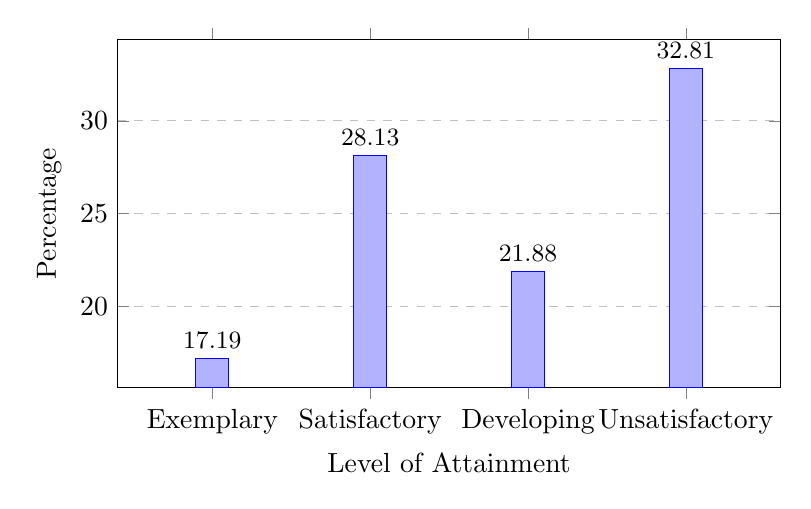
\begin{tikzpicture}
    \begin{axis}[
        ybar,
        width=10cm,
        height=6cm,
        enlarge x limits=0.2, 
        xlabel={Level of Attainment},
        ylabel={Percentage},
        symbolic x coords={Exemplary, Satisfactory, Developing, Unsatisfactory},
        xtick={Exemplary, Satisfactory, Developing, Unsatisfactory}, 
        xtick distance=0.1, 
        ymajorgrids=true,
        grid style=dashed,
        nodes near coords, % Display numbers near bars
        every node near coord/.append style={font=\small, text=black}, 
        bar width=12pt, 
    ]
    \addplot coordinates {(Exemplary, 17.19) (Satisfactory, 28.13) (Developing, 21.88) (Unsatisfactory, 32.81)};
    \end{axis}
    \end{tikzpicture}
     \\
\\
\\
\textbf{Part IV – Analysis.} \\
\\
\parbox{\textwidth}{\raggedright aFunction effectively as a member or leader of a team engaged in activities appropriate to the program’s discipline. Function effectively as a member or leader of a team engaged in activities appropriate to the program’s discipline. Function effectively as a member or leader of a team engaged in activities appropriate to the program’s discipline. Function effectively as a member or leader of a team engaged in activities appropriate to the program’s discipline. Function effectively as a member or leader of a team engaged in activities appropriate to the program’s discipline. Function effectively as a member or leader of a team engaged in activities appropriate to the program’s discipline. Function effectively as a member or leader of a team engaged in activities appropriate to the program’s discipline. Function effectively as a member or leader of a team engaged in activities appropriate to the program’s discipline.Function effectively as a member or leader of a team engaged in activities appropriate to the program’s discipline. Function effectively as a member or leader of a team engaged in activities appropriate to the program’s discipline.}
\end{document}
